%%%%%%%%%%%%%%%%%%%%%%%%%%%%%%%%%%%%%%%%%%%%%%%%%%%%%%%%%%%%%%%%%%%%%%%%%%%%%%%
%%                                                   FORWARD BACKWARD ASYMMETRY
%%%%%%%%%%%%%%%%%%%%%%%%%%%%%%%%%%%%%%%%%%%%%%%%%%%%%%%%%%%%%%%%%%%%%%%%%%%%%%%
%%                       the chapter about the AFB and the sin2theta extraction



%______________________________________________________________________________
%                     Messung der Asymmetrie und des schwachen Mischungswinkels
\chapter{Messung der Asymmetrie und des schwachen Mischungswinkels}
\label{afb}

\begin{quote}
    The abstact comes last
\end{quote}



%______________________________________________________________________________
%                                                      Datensätze und Selektion
\section{Datensätze und Selektion}
\label{afb:selection}

% + benutzter Datensatz
% + Selektion / Akzeptanz
% + Benutzte Gewichte

% + Kontroll-Plots der Masse / Winkelverteilung / Phi

Die Messung der Vorwärts-Rückwärts Asymmetrie und die anschließende Extraktion
des schwachen Mischungswinkels basiert, wie schon die vorangegangene
Energiekalibration, auf dem vollen Datensatz des Jahres 2012 mit $8\TeV$
Schwerpunktsenergie und einer integrierten Luminosität\footnote{nach Anwendung
der \ac{GRL}} von $20.3\fb^{-1}$. Zur Selektion der interessanten Ereignisse
werden die in Abschnitt \ref{data_sim_selection:selection} beschriebenen
Schnitte angewendet (siehe Tabelle \ref{tab:data_selection}), wobei die
Unterteilung der Ereignismenge nach solchen mit Beteiligung von
Vorwärts-Elektronen (CF) und reinen Zentral-Zentral Ereignissen (CC) zunächst
beibehalten wird. Die Analyse und Messung wird dann in diesen beiden Kanälen
zuerst getrennt durchgeführt und abschließend zu einem kombiniertem Ergebnis
zusammengefasst.
\begin{table} [h]
    \centering
    \begin{tabular}{|l|r|r|}
        \hline
        & \multicolumn{2}{|c|}{Elektronkandidaten}   \\
        \textbf{Schnitt} & \textbf{CC} & \textbf{CF} \\  % escale CF
        \hline\hline
        \ac{GRL}           & 389741202 & 389741202   \\  % 3954702112
        Detektor Status    & 389740981 & 389740981   \\  % 3945153030
        Trigger            & 158129884 & 158129884   \\  % 1402546381
        primärer Vertex    & 157901943 & 157901943   \\  % 1400899527
        Pseudorapidität    & 149728397 & 122396071   \\  % 1328016208
        Transversal-Impuls &  63811039 &   8342860   \\  %  498956943
        Autor              &  17186000 &   7841721   \\  %  378463236
        ID                 &   4326530 &    995073   \\  %   76603185
        Ladung             &   4266425 &  (995073)   \\  %           
        OQ                 &   4245028 &    988991   \\  %   75178238
        \hline
    \end{tabular}
    \caption[Anzahl der Elektronkandidaten in Daten für CC und CF Selektion]
        {Anzahl der Elektronkandidaten in Daten nach für CC und CF Selektion.
        Die Auflistung ist inklusiv, d.h. untere Schnitte enthalten implizit
        alle vorangegangenen Schnitte. \development (check numbers with
        calibration)}
    \label{tab:data_selection}
\end{table}
Auf alle Elektronkandidaten im Datensatz werden zuvor noch die entsprechenden
Kalibrationfaktoren für die Energie angewendet (siehe Kapitel
\ref{data_sim_selection:data} und \ref{energy_calibration}), sodass die
Selektion auf kalibrierten Energiewerten stattfinden kann.

Zur simulationsseitigen Beschreibung des Signalprozesses
$pp \rightarrow \gamma^*/Z(e^+e^-) + X$, also dem elektroschwachen Zerfall
eines $Z$-Bosons bzw. virtuellen Photons in ein Elektronpaar\footnote{auch hier
wird der Begriff \textit{Elektron} wieder synonym für Teilchen und Antiteilchen
verwendet}, wird das von \textsc{Powheg+Pythia} generierte Drell-Yan
Monte-Carlo verwendet (siehe Kapitel \ref{used_mc_samples}). Es werden
identische Selektionkriterien, wie auf den Daten angewendet, wobei die Energie
der Elektronkandidaten zuvor einer Auflösungskorrektur unterzogen wird. Dabei
wird eine künstliche Verschmierung der Energie eingeführt, um die oftmals zu
optimistisch angenommene Energieauflösung im Monte-Carlo nachträglich zu
korrigieren\footnote{weitere Details siehe Kapitel \ref{energy_calibration}}.
Zudem wird für jedes selektierte Ereigniss ein spezifisches Gewicht errechnet,
mit dem dieses Ereignis bei der Erstellung von statistischen Verteilungen
beträgt. Es gehen hierbei Ereignis spezifische, sowie Elektron spezifische
Korrekturfaktoren in die Bildung dieses Gewichtes ein, deren Ursprung und
Benutzung in Kapitel \ref{mc_corrections} motiviert wurde. Zusammengefasst
ergeben sich die Gesamtgewichte zu
\begin{align}
    w_\text{event}^\text{CC} &= w_\text{pu} \cdot w_\text{kFactor} \cdot
        w_\text{vtx} \cdot w_\text{gen} \cdot \prod_{i=1,2} w_{\text{ID},i}
        \cdot w_{\text{spur},i} \cdot w_{\text{trigger},i}
        \\[2pt]
    w_\text{event}^\text{CF} &= w_\text{pu} \cdot w_\text{kFactor} \cdot
        w_\text{vtx} \cdot w_\text{gen} \cdot w_{\text{ID},1} \cdot
        w_{\text{ID},2} \cdot w_{\text{spur}} \cdot w_{\text{trigger}}
\end{align}
wobei der Index $i$ in \ac{CC} Ereignissen verdeutlicht, dass die
entsprechenden Korrekturfaktoren für beide Zentral-Elektronen separat eingehen.
In \ac{CF} Ereignissen findet diese Unterscheidung nur für den Faktor der
Identifikationseffizienz statt, da die beiden übrigen Effizienzkorrekturen
nicht für Vorwärts-Elektronen definiert sind.

Zur Abschätzung der Beiträge von Untergrundprozessen wird eine Kombination aus
Simulation und datengestützter Betimmung verwendet. Beide Aspekte werden im
Folgenden näher erläutert und deren Anteil an den selektierten Ereignissen
quantifiziert.



\subsection{Simulierte Untergrundbeiträge}
\label{afb:monte_carlos}

% + Benutzte Monte-Carlos

Neben dem Drell-Yan Prozess mit zwei Elektronen im Endzustand gibt es
zahlreiche weitere Prozesse, die eine ähnliche Signatur im Detektor zeigen und
deshalb von der oben beschriebenen Selektion inkludiert werden. Das Prinzip der
Abschätzung dieser Untergrundbeiträge mittels Simulationen, beruht auf der
Erstellung von Monte-Carlos für jeden relevanten, d.h. möglicherweise
beitragenden, Prozess und der anschließenden Anwendung der selben
Selektionsschnitte, analog zur Selektion in realen Daten. Die aus den
verbleibenden Ereignissen gewonnenen Verteilungen\footnote{Selbstverständlich
ist hierbei auch die mit Gleichung (\ref{eq:mc_scaling}) beschriebene
Skalierung auf Luminosität erforderlich} quantifizieren sodann den Beitrag des
jeweilig betrachteten Prozesses. Alle hier nachstehend aufgeführten Monte-Carlo
Simulationen sind mit ihren Charakteristika bereits in Kapitel
\ref{used_mc_samples} eingeführt worden und werden hier vom motivierenden
Standpunkt der Untergrundabschätzung aus betrachtet.

Einen der größten Beiträge zum Untergrund stellt die Produktion und der Zerfall
eines Top-Antitop Quarkpaares dar (im Folgenden mit \texttt{ttbar} bezeichnet).
Topquarks haben ein Verzweigungsverhältnis von beinahe 100\% für den Zerfall in
ein $b$-Quark und ein $W$-Boson. Solche Ereignisse passieren die Selektion,
wenn entweder beide $W$-Bosonen leptonisch in jeweils ein Elektron und ein
Antielektronneutrino zerfallen, oder Jets aus den $b$-Quarks bzw. dem
hadronischen Zefall eines oder beider $W$-Bosonen fälschlicherweise als
Elektronen rekonstruiert werden. Ähnlich, jedoch in sehr viel geringerem
Umfang, trägt auch die Produktion eines einzelnen Top-Quarks und dessen
konsekutiver Zerfall zum Untergrund bei (nachfolgend \texttt{SingleTop}
genannt). Die relevanten Zerfallskanäle sind dieselben, jedoch muss nun
folgerichtig stets ein irrtümlich identifizierter Jet beteiligt sein.

Der leptonische Zerfall eines $W$-Bosons in ein Elektron und ein
Antielektronneutrino spielt auch für sich allein betrachtet eine wichtige
Rolle. Der Wirkungsquerschnitt für die Produktion eines $W$-Bosons ist um
einiges größer, als für den untersuchten Signal-Prozess. Wie schon beim
Topquark-Untergrund tragen hier Ereignisse bei, in denen ein Jet von den
Rekonstruktionsalgorithmen als Elektron erkannt wird. Auch der verwandte
Prozess des $W$-Zerfalls in ein Tauon und das entsprechende Antineutrino
liefern einen Beitrag, da Tauonen eine Verzweigungsverhältnis von rund $18\%$
für den Zerfall in ein Elektron aufweisen. Zusammengefasst werden alle
Untergründe dieser Art in der Folge mit \texttt{WJets} gekennzeichnet.

Ein weitere Kontribution zum Untergrund entstammt der Produktion von $WW$-,
$WZ$- und $ZZ$-Bosonpaaren. Hier finden sich im Endzustand häufig zwei oder
Elektronen, sodass die Wahrscheinlichkeit hoch ist, dass diese die
kinematischen Anforderungen erfüllen und sie Selektion passieren können.
Natürlich kommen hierbei auch wieder falsch identifizierte Jets aus
hadronischen Zerfällen zum Tragen. Im folgenden werden aber alle Prozesse
dieser Art, also solche, die die Produktion eines der genannten Bosonpaare
beinhalten, unter dem Begriff \texttt{Diboson} zusammengefasst.

Einen sehr geringen, wenn auch nicht vernachlässigbaren Anteil liefert der
Drell-Yan Prozess selbst, nämlich beim Zerfall in ein $\tau^+\tau^-$-Paar
(\texttt{DYtautau}). Wie schon beim $W$-Untergrund erwähnt können Tauonen in
Elektronen zerfallen, weshalb dieser Prozess in der Lage ist, von der Selektion
erfasst zu werden.

Abbildung \ref{fig:elec_kinematics} zeigen die
Verteilungen des Transversalimpulses $p_T$ und der Pseudorapidität $\eta$ für
die einzelnen Elektronen nach Anwendung der Selektionsschnitte. Die
Untergrundbeiträge sind entsprechend der oben eingeführten Kürzel
(\texttt{ttbar},...) farbig gekennzeichnet und aufeinandergestapelt
dargestellt.

\begin{figure}[hp]
    \centering
    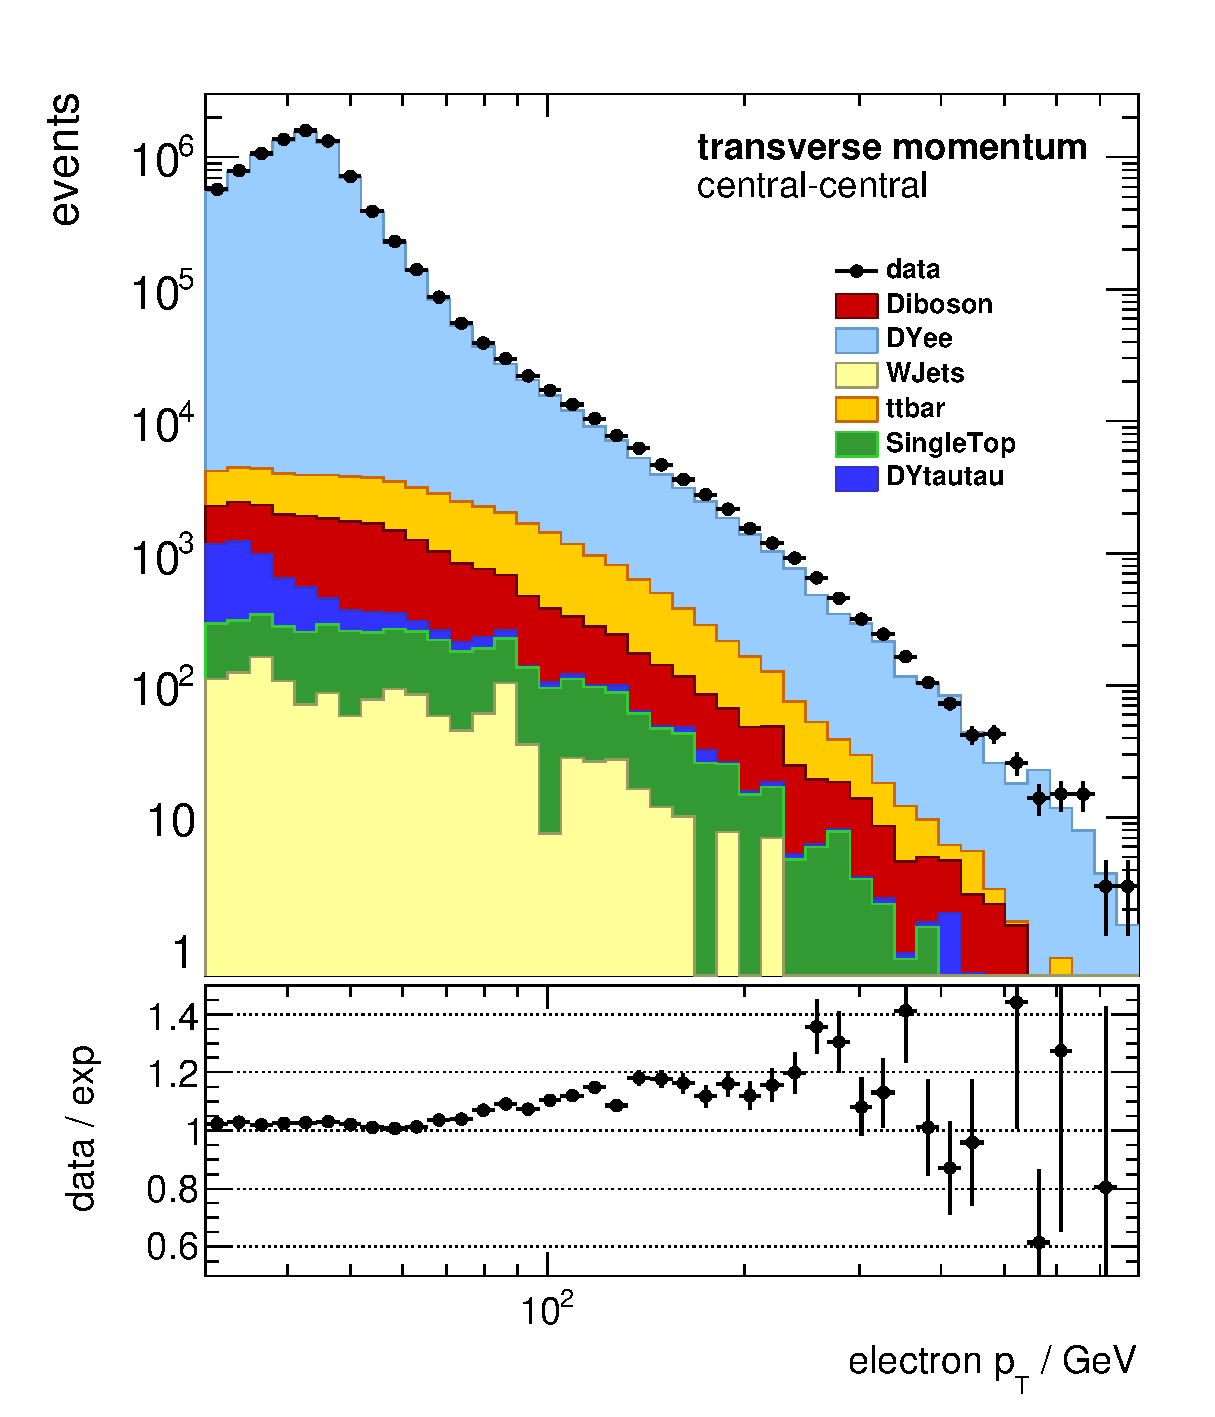
\includegraphics[width=0.48\textwidth]{plots/pt_cc}
    \hfill
    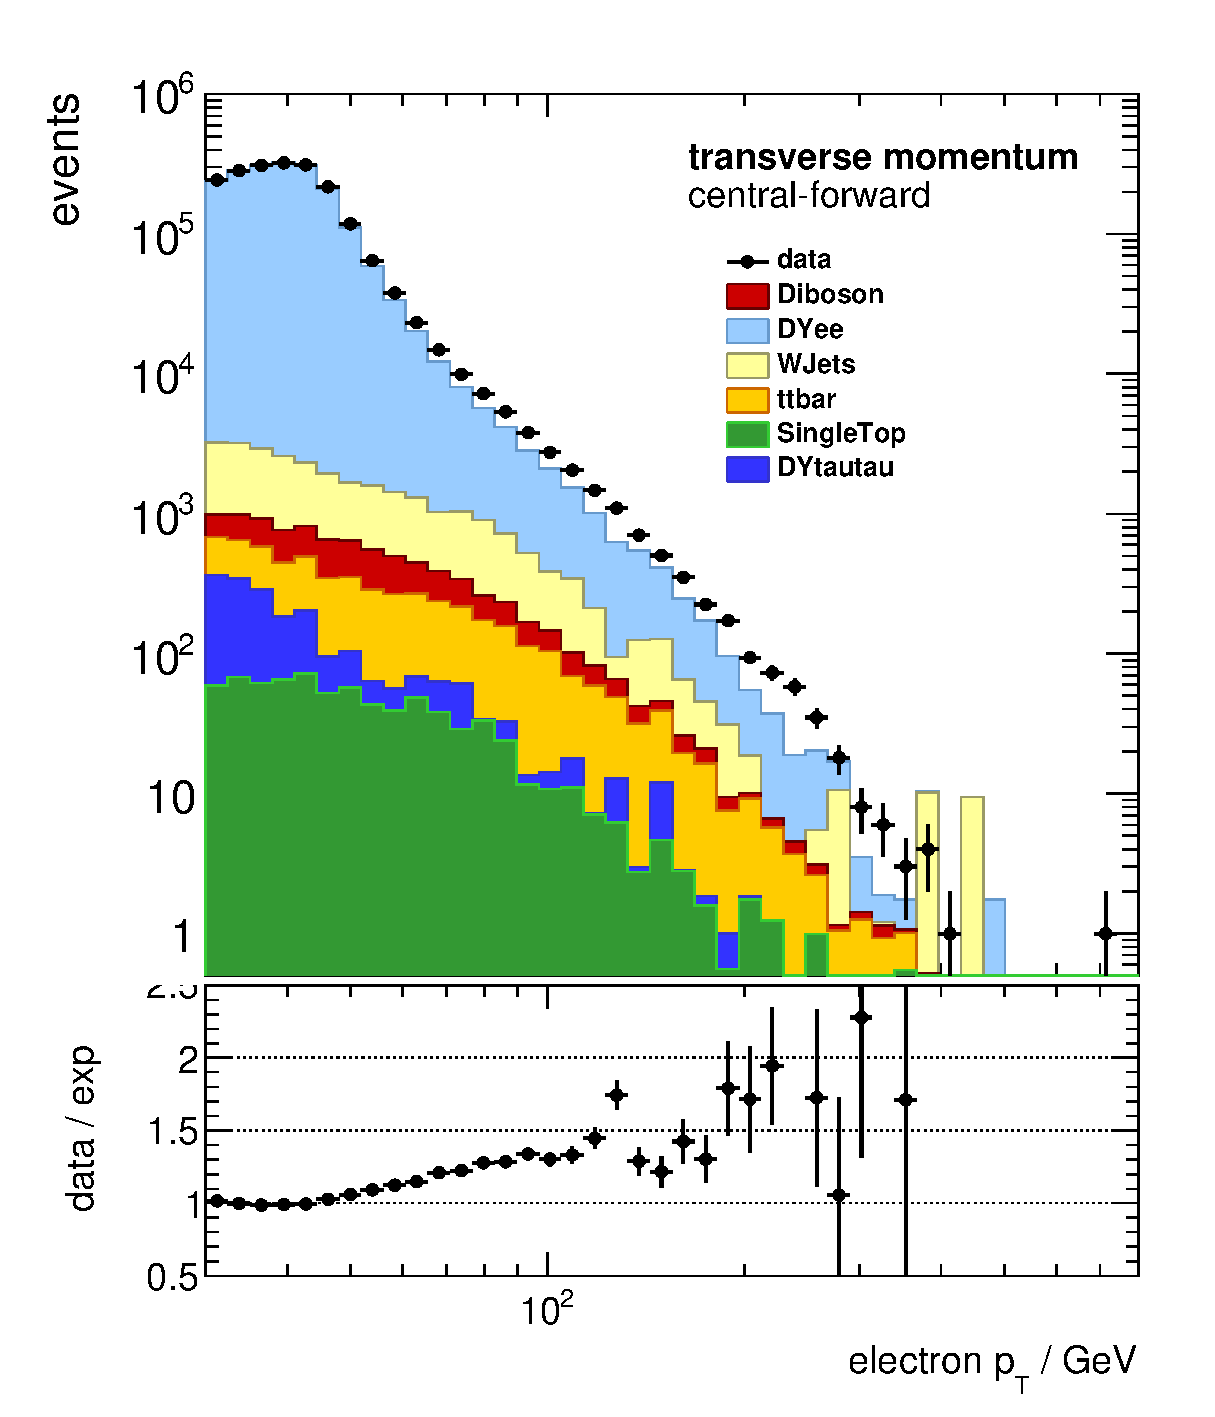
\includegraphics[width=0.48\textwidth]{plots/pt_cf}

    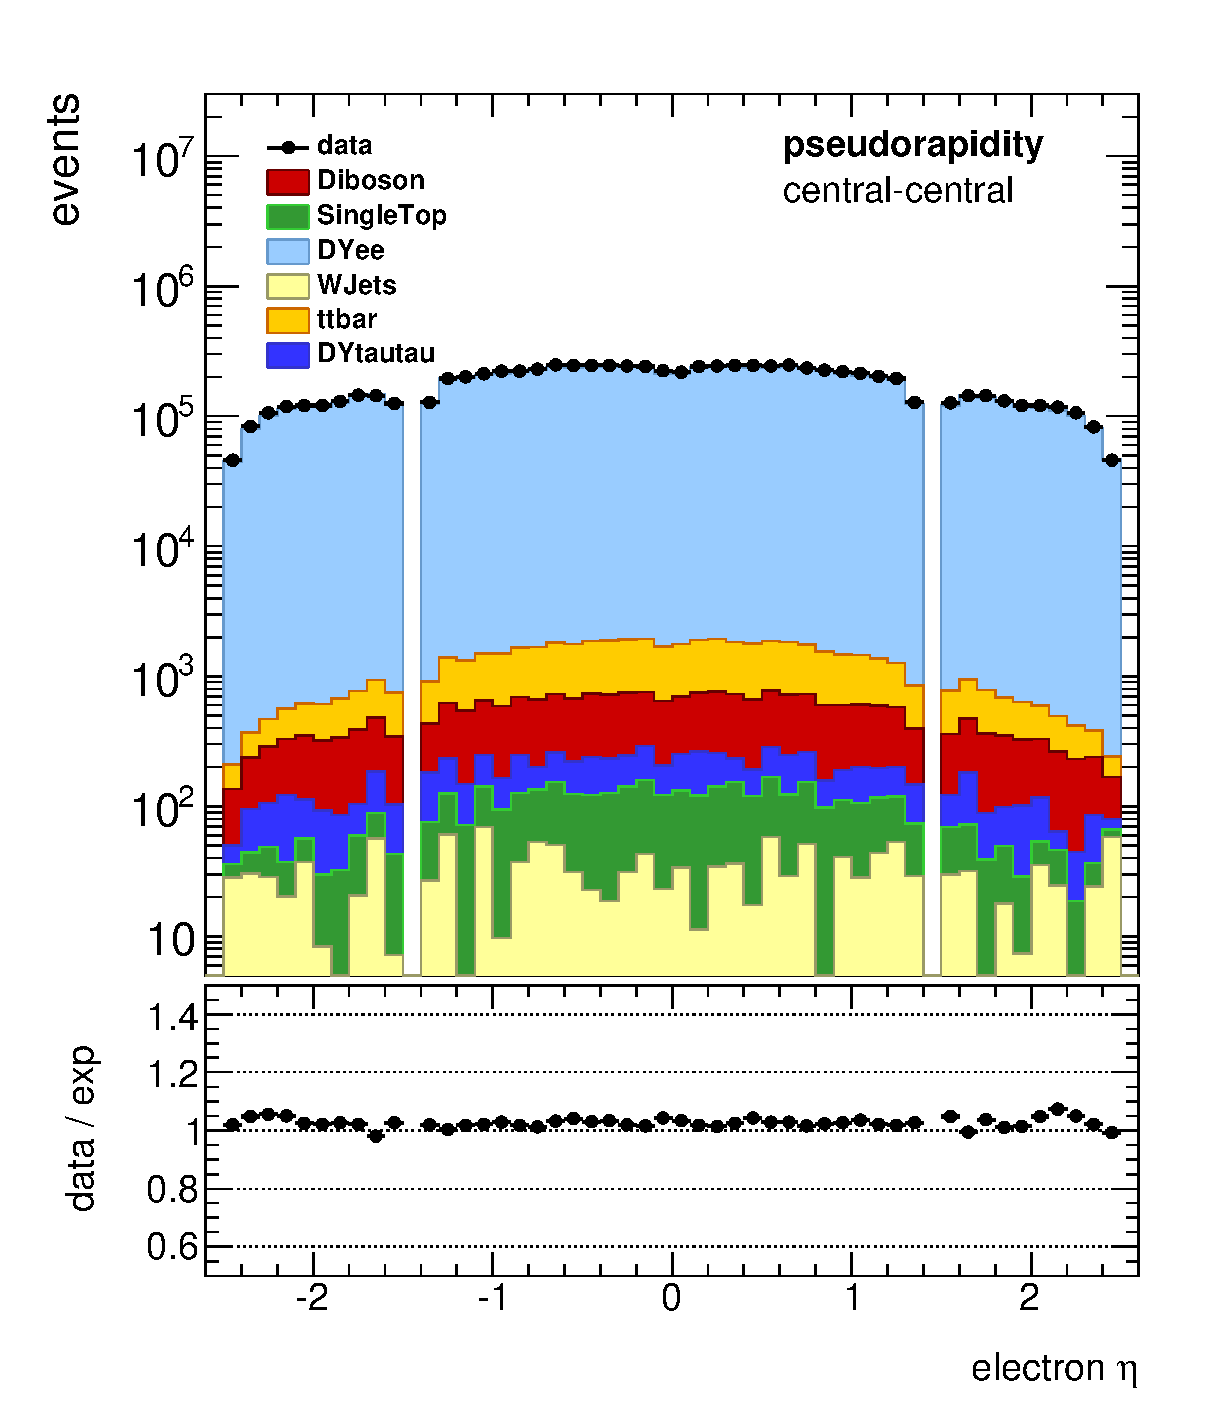
\includegraphics[width=0.48\textwidth]{plots/eta_cc}
    \hfill
    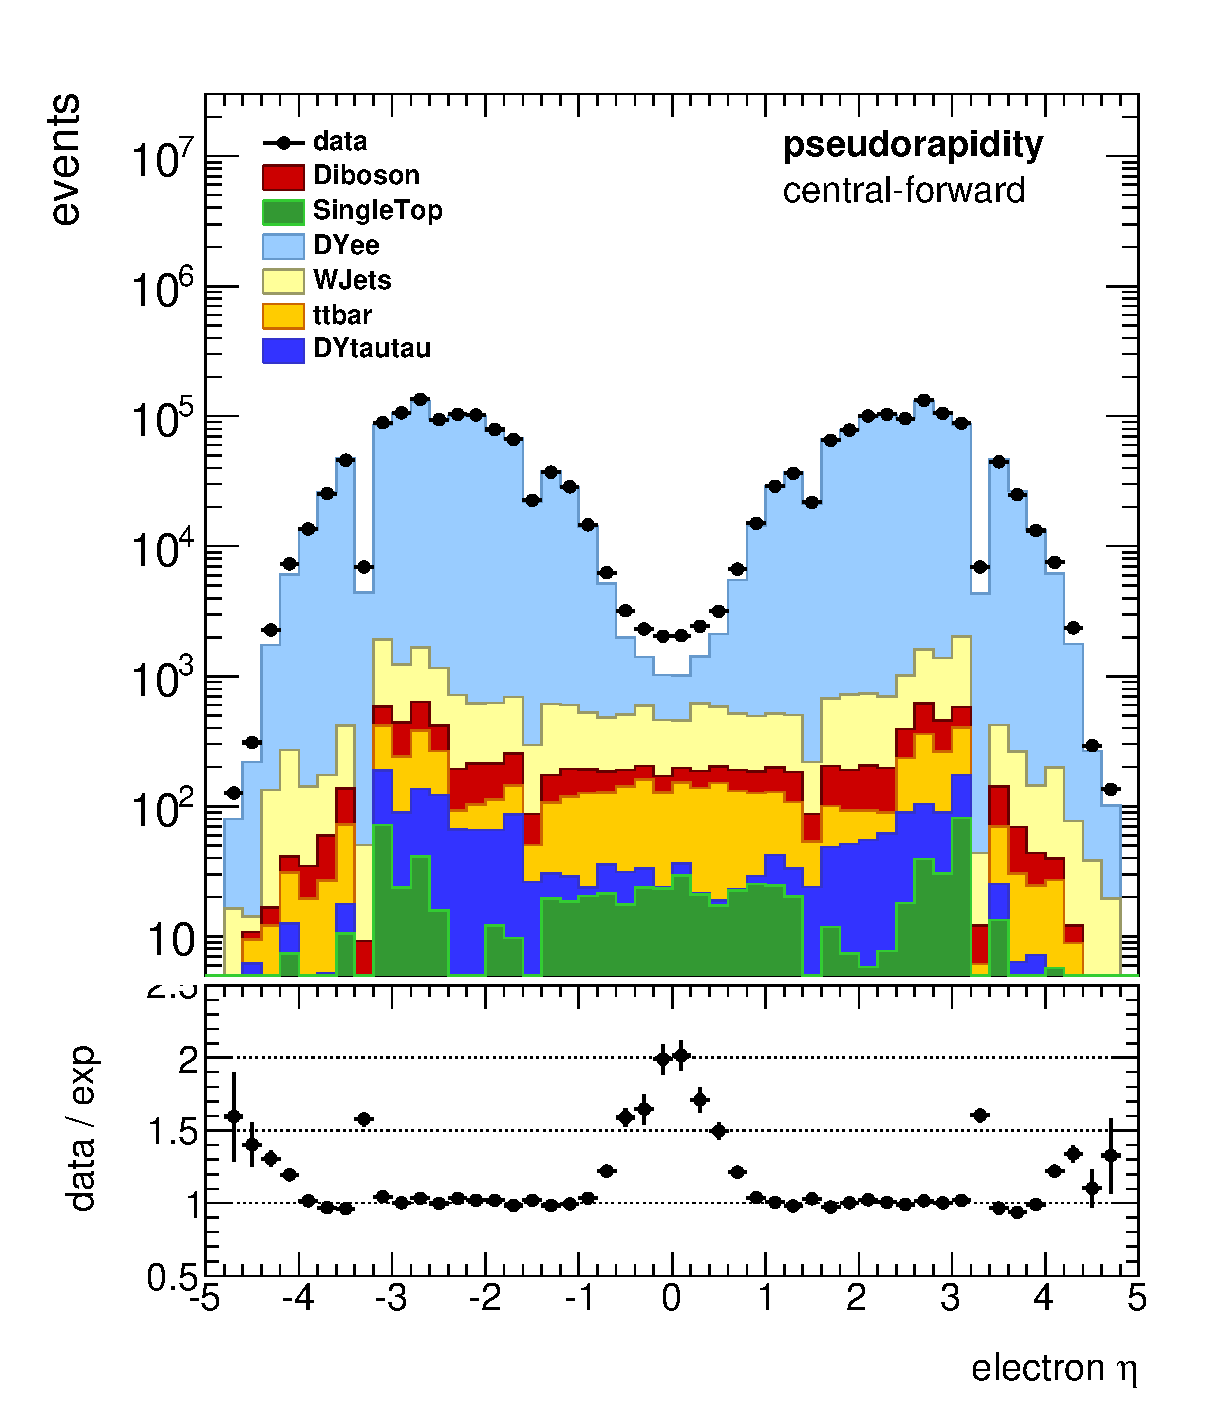
\includegraphics[width=0.48\textwidth]{plots/eta_cf}
    \caption[Kinematische Verteilungen der Elektronen nach Selektion in \ac{CC}
        und \ac{CF}]
        {Kinematische Verteilungen der Elektronen nach Selektion in \ac{CC}
        (links) und \ac{CF} (rechts) für den Transversalimpuls (oben) und die
        Pseudorapidität (unten). Der Quotient aus Daten und dargestellter
        Untergundsumme ist jeweils unter den Histogrammen gezeigt.}
    \label{fig:elec_kinematics}
\end{figure}

Erwartungsgemäß zeigen die Verteilungen des Transversalimpulses in Daten ein
Maximum bei etwa $45\GeV$, also gerade der halben Masse des $Z$-Bosons
und einen daran anschließenden starken Abfall mit steigendem Transversalimpuls.
Ein analoges Verhalten wird bei der Simulation des Signalprozesses
(\texttt{DYee}) beobachtet. Die übrigen Untergrundspektren weisen ebenfalls den
erwarteten Verlauf eines mit größer werdendem $p_T$ abfallendes Spektrum auf,
zeigen dagegen aber keine ausgeprägte Extremstelle. Einzige Ausnahme dabei
stellt das \texttt{DYtautau} Spektrum dar, welches ein solches Maximum
unterhalb von $45\GeV$ aufweist. Die Verschiebung dieses Maximums unter die
halbe $Z$-Masse liegt darin begründet, dass die Elektronen in diesem Prozess
aus den direkten Zerfallsprodukten des Bosons, den Tauonen, hervorgehen und
folglich nicht deren vollen Impuls tragen.

Desweiteren fällt beim Vergleich zwischen den Spektren für \ac{CC}- und
\ac{CF}-Selektion auf, dass sich der Umfang der Untergrundbeiträge deutlich 
unterscheidet. Am deutlichsten zeigt sich dies beim \texttt{WJets}
Untergrund, der in \ac{CF} den größten Beitrag zum Untergrund darstellt,
während dessen Rolle in \ac{CC} von geringer Bedeutung ist. Die Ursache
hierfür ist, dass im Vorwärts-Bereich die Wahrscheinlichkeit der
Fehlidentifikation eines Jets als Elektron wesentlich höher ist, als im
Zentral-Bereich, was unter anderem auf die fehlende Spurinformation im
Vorwärts-Bereich zurückzuführen ist\footnote{siehe hierzu auch Kapitel \ref{}}.

Unter jeder Abbildung ist zudem der Quotient aus der Datenverteilung und der
Summe alle Monte-Carlos (Untergründe + Signal) dargestellt. Diese zeigt, gerade
in Bereichen mit hohem Transversalimpuls eine deutliche Diskrepanz. Hierin
verbirgt sich ein weiterer bisher nicht betrachteter Untergundbeitrag der durch
Prozesse der \ac{QCD} bestimmt ist und deshalb nur schwer simulierbar ist. Die
Methode zur Abschätzung dieses Beitrags ist Gegenstand des nachfolgenden
Abschnitts.

Bei der Betrachtung der Spektren der Pseudorapidität ist zunächst zu beachten,
dass diese auf unterschiedlichen Skalen, entsprechend der jeweiligen Schnitte
in der Selektion, aufgetragen sind. In beiden Selektionen zeigen sich
natürlicherweise um Null symmetrische Spektren und die Exklusionen der
Kalorimeter Übergangsregionen ist deutlich sichtbar. Die Form der Verteilungen
im \ac{CC} Kanal zeigen einen leicht nach außen abfallenden Verlauf, während im
\ac{CF} Kanal zwei deutliche Erhebungen auszumachen sind. Diese haben ihr
Maximum bei $\eta\approx\pm 2,5$, was dem Übergang zwischen Zentral- und
Vorwärts-Bereich entspricht. Die Ausprägung dieser Struktur ist den
angewendeten Selektionkriterien geschuldet, die den Öffnungswinkel
zwischen den beiden Elektronen in der \ac{CF}-Selektion
einschränken\footnote{die \ac{CF} Selektion unterdrückt Ereignisse mit
Öffnungswinkeln $\theta \approx \pi$}. Die Untergrundbeiträge tragen hier
selbstverständlich im gleichen Maße bei, wie schon bei den Spektren des
Transversalimpulses erläutert. Schaut auf den jeweils darunter dargestellten
Quotienten aus Daten und Monte-Carlo, lässt sich etwas über den bisher
vernachlässigten Beitrag des \ac{QCD} Untergrundes etwas lernen. So resultiert
dessen Ignorieren im \ac{CC}-Kanal zu einem breiten, den vollen $\eta$-Bereich
abdeckenden Überschuss an Datenereignissen, während im \ac{CF}-Kanal diese
Überschüsse auf die Randbereiche ($|\eta| > 4,0$) und um das Zentrum ($\eta=0$)
konzentrieren.



\subsection{Datengestützte Untergrundabschätzung}
\label{afb:multijet}
Nachdem im vorangegangenen Abschnitt die Untergrundbeiträge simulierbarer
Prozesse untersucht wurden, steht nun die Examinierung der eben bereits
erwähnten Beiträge durch reine Prozesse der starken Wechselwirkung an. Die
Anzahl der möglichen Parton-Konstellationen innerhalb dieser Prozesse ist groß,
jedoch ist allen beitragenden Ereignissen gemein, dass sie mindestens zwei Jets
im Endzustand aufweisen, die irrtümlich als Elektronen rekonstruiert werden,
weshalb im Folgenden auch von \texttt{MultiJet} Untergrund gesprochen wird.

Zu dessen Abschätzung wird die sogenannte \textit{ReverseID}-Methode (vom engl.
reverse, umgekehrt) benutzt. Das Grundprinzip dabei sieht vor, einen neuen Satz
von Selektionsschnitten zu erstellen, der sich gegenüber der normalen
Signalselektion lediglich in der Umkehrung der Identifiaktionskriterien
unterscheidet. Das heißt konkret man verlangt anstelle einer bestimmten
Identifikationsstufe\footnote{z.B. \textit{tight++} (siehe Kapitel
\ref{})} für Elektronkandidaten die darunter liegende Stufe und fordert
gleichzeitig das Scheitern des ursprünglichen Kriteriums. Abbildung
\ref{fig:reverseID} veranschaulicht dies.
\begin{figure}[h]
    \centering
    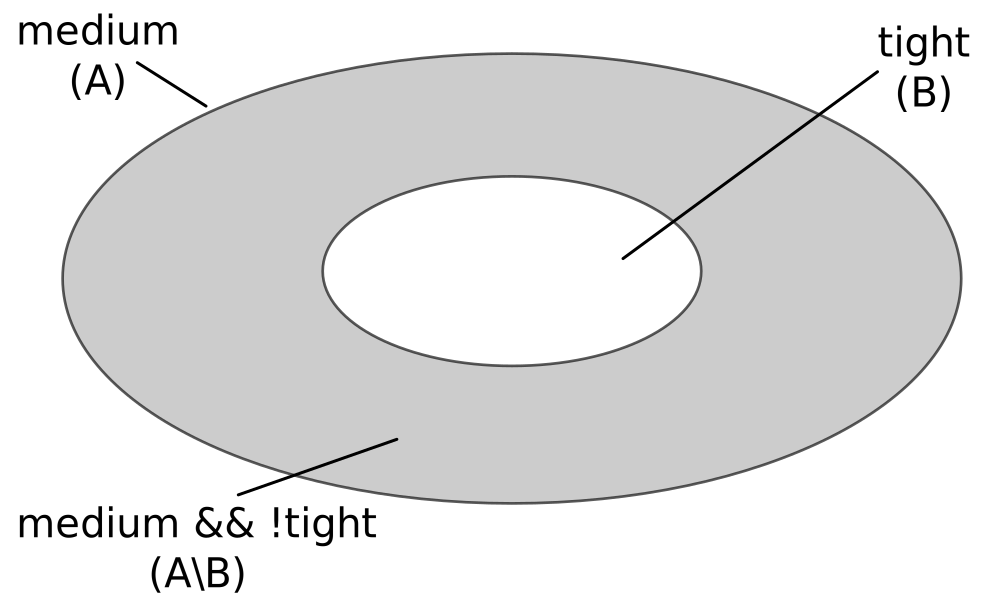
\includegraphics[width=0.5\textwidth]{img/reverseID}
    \caption[Mengentheoretische Darstellung der Selektion in der
        ReverseID-Methode]
        {Mengentheoretische Darstellung der Selektion in der ReverseID-Methode.
        \textbf{Signalselektion:} $B\quad$ \textbf{ReverseID-Selektion:}
        $A \backslash B$}
    \label{fig:reverseID}
\end{figure}
Da die Menge der Elektronen, die eine bestimmte ID-Stufe erfüllen stets eine
Teilmenge der darunterliegenden Stufe ist, ist die Menge der mit ReverseID
selektierten Elektronen statistisch unabhängig von der ursprünglichen Menge.
Auf den vollen Datensatz angewendet ist das Ziel dabei die Auslese jener
Ereignisse mit signalähnlichen Jets, die eine hohe Wahrscheinlichkeit haben als
Elektronen identifiziert zu werden.

Man trifft nun die Annahme, dass die statistische Verteilung dieser Ereignisse
geeignet ist, um die Form des \texttt{MultiJet} Untergrundbeitrages zu
repräsentieren, lediglich die Skalierung bleibt noch zu bestimmen. Letzteres
wird erreicht, indem man alle simulierten Untergünde (s.o.), das Signal
Monte-Carlo und die \texttt{MultiJet} Verteilung aufaddiert und diese Summe
mittels eines freien Skalierungsfaktors für die \texttt{MultiJet} Verteilung an
die beobachtete Datenverteilung anpasst.

Um Doppelzählungen mit fehlrekonstruierten Jets aus bereits simulierten
Untergründen (siehe voheriger Abschnitt) auszuschließen wird die ReverseID
Selektion ebenfalls auf alle bereits verwendeten Monte-Carlos angewandt und
deren Beitrag von der aus Daten erzeugten Verteilung subtrahiert.

In dieser Arbeit wird für die Signalselektion die Identifikationsstufe
\textit{tight++} für Zentral- bzw. \textit{fwdTight} für Vorwärts-Elektronen
verwendet. Dementsprechend werden für die ReverseID-Methode die folgenden
ID-Kriterien gefordert:
\begin{table}[h]
    \centering
    \begin{tabular}{
                        |c|
                        >{\centering\arraybackslash}p{45mm} |
                        >{\centering\arraybackslash}p{45mm} |
                   }
        \hline
        \bf{Bereich} & \bf{Signal Selektion} & \bf{ReverseID Selektion} \\
        \hline\hline
        Zentral  & \it{tight++}  & \textit{medium++} $\wedge$!\it{tight++} \\
        \hline
        Vorwärts & \it{fwdTight} & \textit{fwdMedium} $\wedge$!\it{fwdTight} \\
        \hline
    \end{tabular}
    \caption[Identifikations Kriterien der ReverseID-Methode]
        {Identifikations Kriterien der ReverseID-Methode. Ein '!' meint eine
        logische Negierung.}
    \label{tab:reverseID}
\end{table}

Zur Bestimmung des Skalierungsfaktors wird das, bereits für die
Kurvenanpassungen der Energiekalibration verwendete, Software-Paket
\textsc{RooFit} (\cite{Verkerke:2003ir}) verwendet. Dieses stellt die
Möglichkeit bereit Histogramme als Anpassungsmodelle zu verwenden. Oben
definierte \texttt{MultiJet} Verteilung wird nun als solches Modell mittels des
freien Skalierungsfakotrs an die Datenverteilung angepasst.

Abbildung \ref{fig:multijet} zeigt das Ergebnis dieser Anpassung im invarianten
Massenspektrum der Elektronpaare für den \ac{CC} und \ac{CF} Kanal.
\begin{figure}[h]
    \centering
    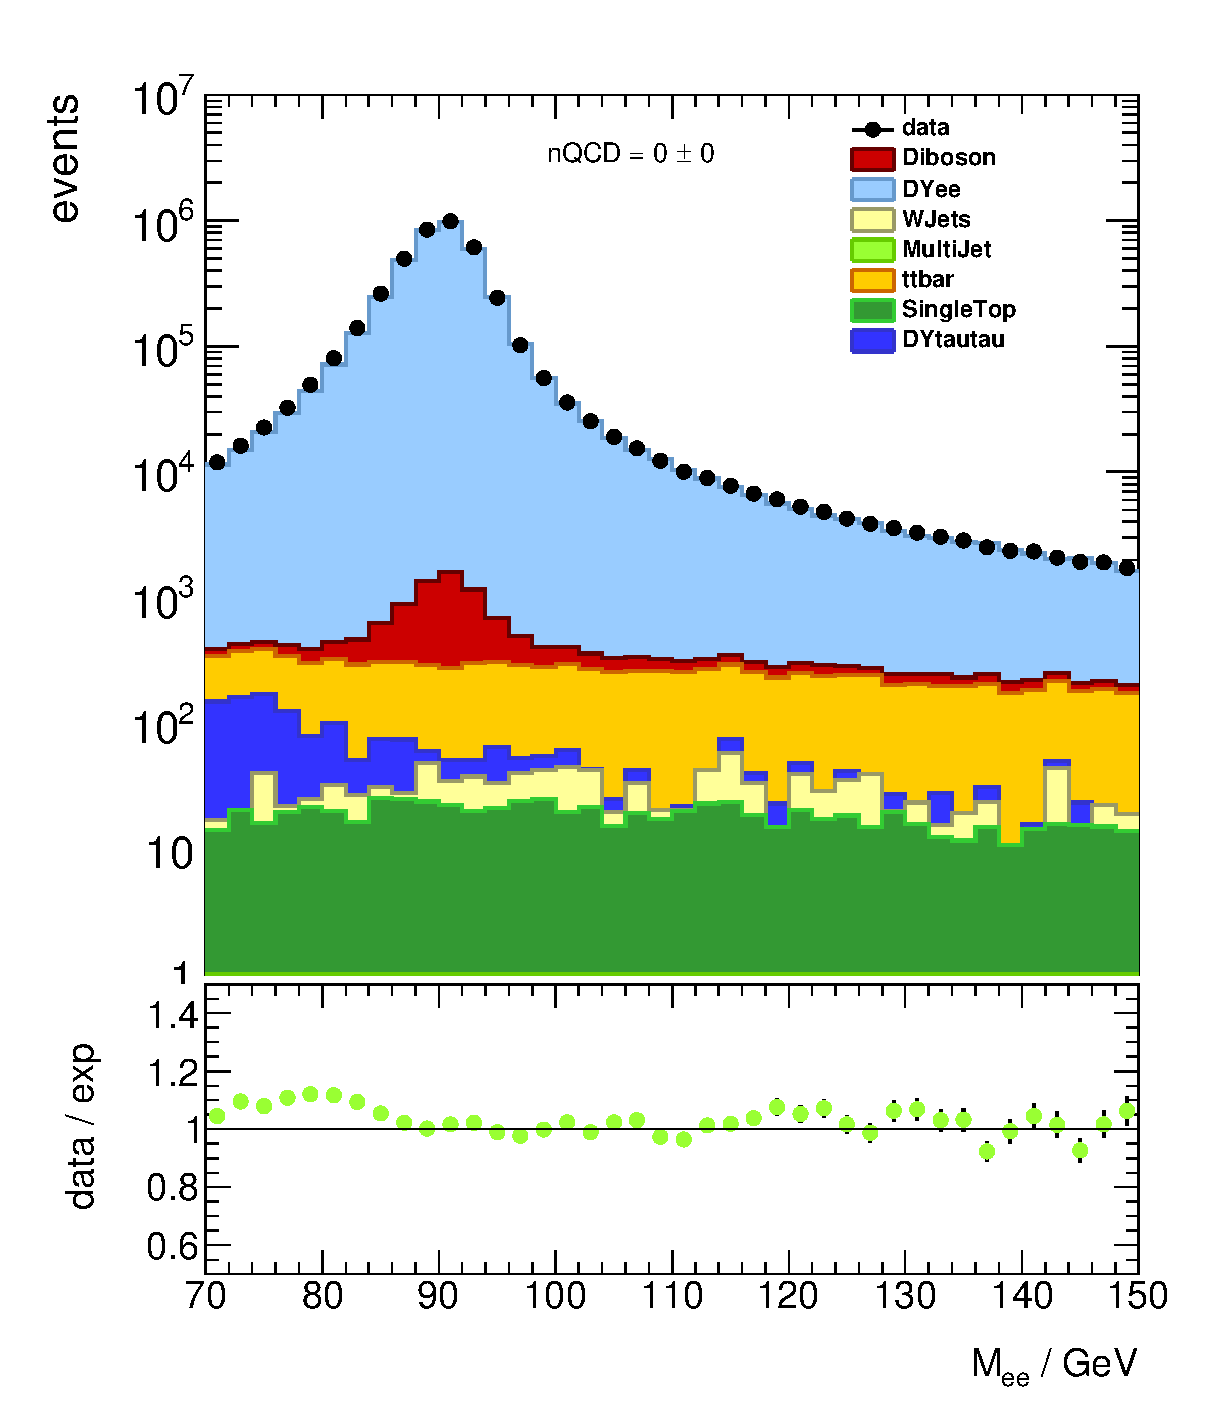
\includegraphics[width=.48\textwidth]{plots/mee_cc}
    \hfill
    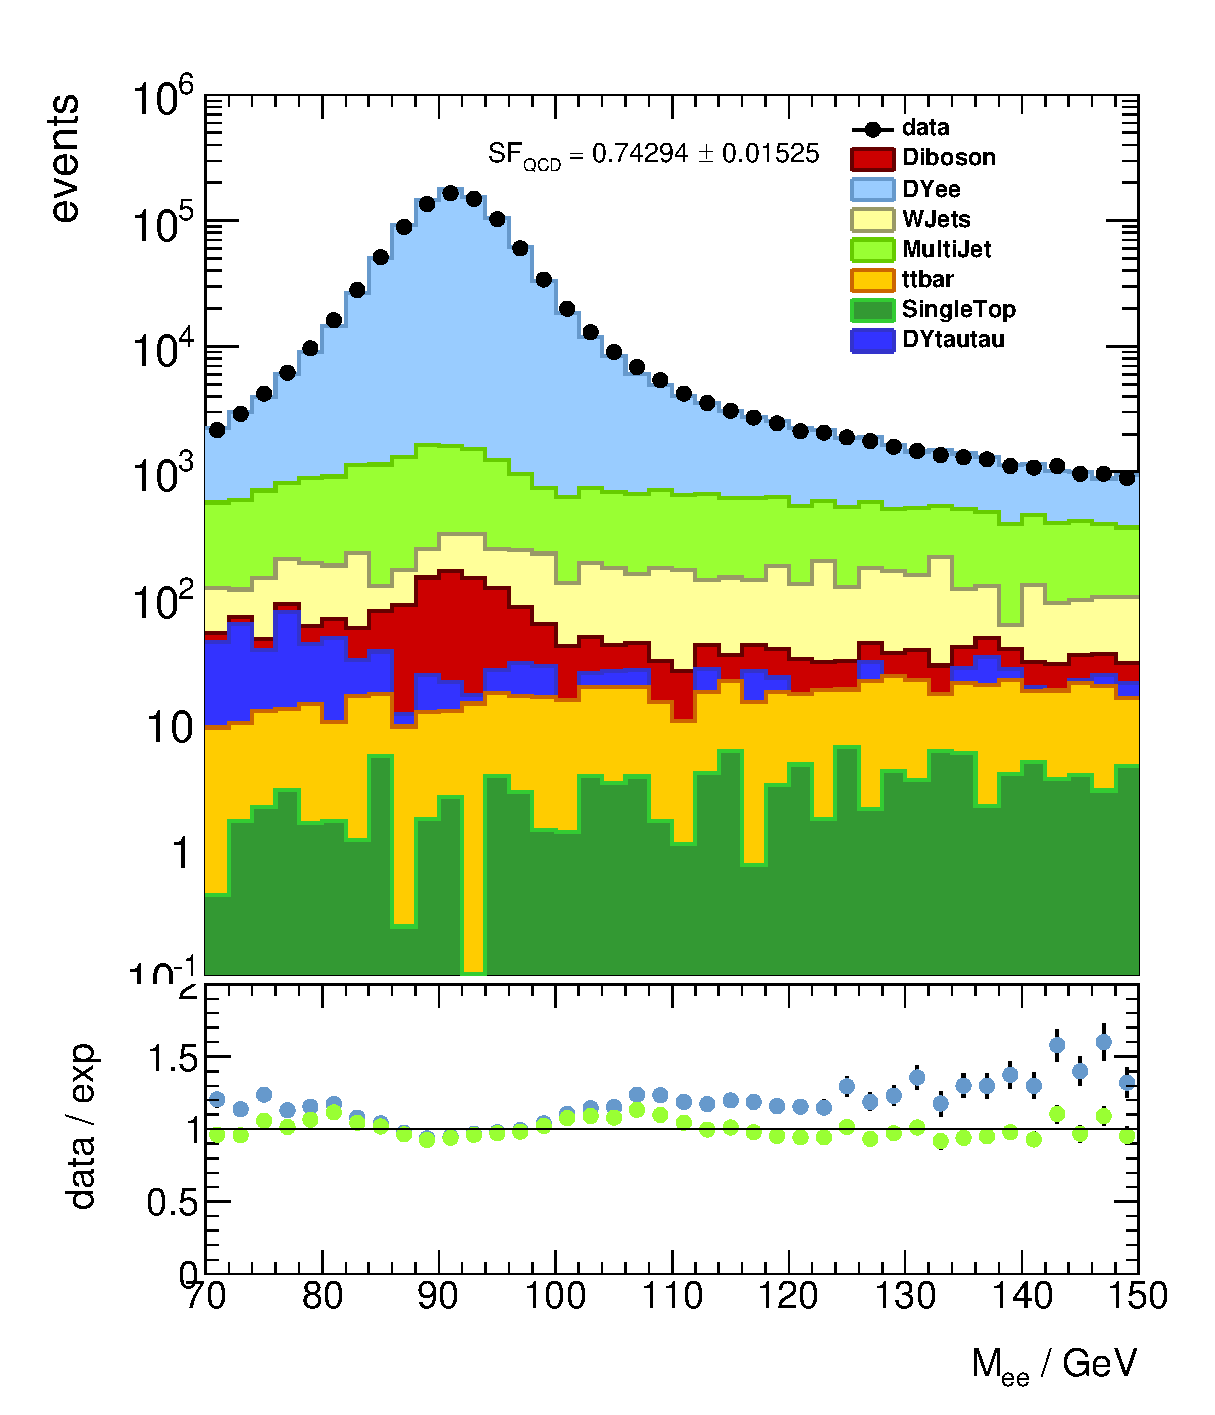
\includegraphics[width=.48\textwidth]{plots/mee_cf}
    \caption[Invariante Masse der Elektronpaare nach MultiJet
        Untergrundanpassung]
        {Invariante Masse der Elektronpaare mit MultiJet Untergrundanpassung
        und allen simulierten Untergründen im \ac{CC}-Kanal (links) und
        \ac{CF}-Kanal (rechts). Die darunter dargestellten Quotienten aus Daten
        und Summe aller Untergründe mit Signal Monte-Carlo zeigen die
        Übereinstimmung vor (blau) und nach (grün) MultiJet-Anpassung.}
    \label{fig:multijet}
\end{figure}
Dabei ist zunächst zu beachten, dass der Bereich der invarianten Masse auf
$70\GeV < M_{ee} < 150\GeV$ eingeschränkt wurde,was zwei Gründe hat. Zum einen
wurde diese Einschränkung schon im Hinblick auf die spätere Extraktion des
schwachen Mischungswinkels vorgenommen und zum anderen weißt die
ReverseID-Methode in höheren Massenbereichen signifkante Defizite auf, welche
deren Anwengung nicht mehr rechtfertigen lassen. So ist zum Beispiel die stetig
abnehmende Statistik ein Problem, viel mehr jedoch die unhaltbare Annahme Jets
würden sich über alle Energien und Bereiche des Detektors stets gleich
verhalten. Alternative Möglichkeiten zur Abschätzung der \ac{QCD}
Untergrundbeiträge werden am Ende des Kapitel diskutiert werden.

Die ermittelten Skalenfaktoren für beide Kanäle sind in Abbildung
\ref{fig:multijet} selbst dargestellt. Im \ac{CF}-Kanal, für den ein großer
Beitrag von \ac{QCD} Ereignissen erwartet wird, zeigt sich dieser mit einem
großen Anteil am Untegrundspektrum. Die Form der \texttt{MultiJet} Verteilung
ist ebenfalls gemäß der Erwartung durchweg flach. Die unter der Verteilung
dargestellten Verhältnisse von Daten zur Summe aller Untergründe und
Signal Monte-Carlo zeigt eine deutliche Verbesserung der Übereinstimmung unter
Hinzunahme des \texttt{MultiJet} Untergrundes. Für den \ac{CC} Kanal zeigt
sich, dass der Beitrag durch \ac{QCD} Ereignisse vernachlässigbar klein
gegenüber alle anderen Untergründen ist, sodass hier kein von Null
verschiedener Faktor ermittelt werden konnte. Die Betrachtung des Verhältnisses
darunter zeigt auch bereits eine hinreichend gute Übereintummung.  Einzig der
Bereich unterhalb von $80\GeV$ weist eine erhebliche Abweichung auf, welches
aber auf ein bekanntes Problem mit der Detektor-Beschreibung innerhalb der
Monte-Carlo Simulation zurückführen ist, welches derzeit von der zuständigen
ATLAS Arbeitsgruppe untersucht wird.



%______________________________________________________________________________
%                                                         Asymmetrie Verteilung
\section{Vorwärts-Rückwärts Asymmetrie Verteilung}
\label{afb:afb}

% + Rohe Verteilung
% + Untergund reduzierte Verteilung
% + Vergleich mit Signal-Simulation

Nach der Abschätzung der Untergrundbeiträge folgt nun die Messung der
Vorwärts-Rückwärts Asymmetrie.




%______________________________________________________________________________
%                          Extraktion des effektiven Schwachen Mischungswinkels
\section{Extraktion des effektiven Schwachen Mischungswinkels}
\label{afb:sin2theta}

% + Extraktionsmethode
%   - Template Erzeugung
%   - Faltung mit Detektoreffekten
% + Extraktion
%   - Template Fits
%   - Closure-Test
%   - Resultate (einzeln und kombiniert)
% + Diskussion
%   - Systematische Betrachtungen
%   - Vergleich mit anderen Experimenten
%   - Ausblick (..., Alternativen zur ReverseID, ...)
 


